\documentclass[10pt,journal]{IEEEtran}
\usepackage{amsmath,amssymb,amsfonts}
\usepackage{xcolor}
\usepackage{pgfplots}
\pgfplotsset{compat=newest}
\usetikzlibrary{shapes, arrows.meta}

\begin{document}

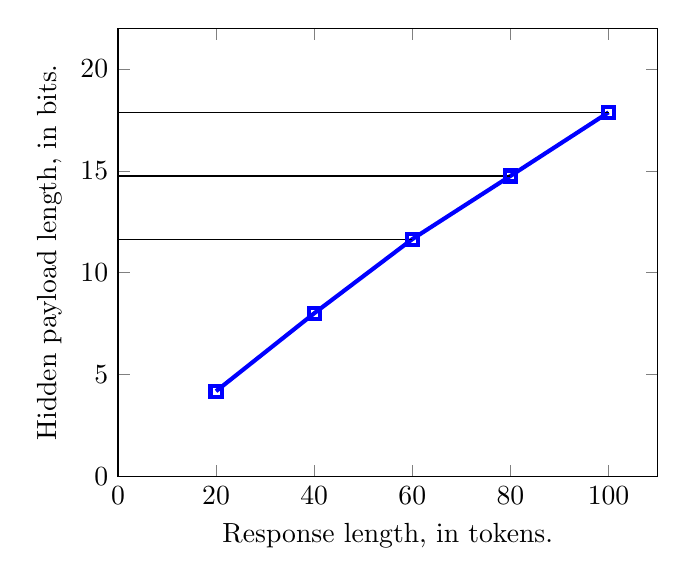
\begin{tikzpicture}
    \begin{axis}[
        xmin=0,xmax=110,
        ymin=0,ymax=22,
        xlabel={Response length, in tokens.},
        ylabel={Hidden payload length, in bits.},
        ]
        \addplot [
            color=blue,
            solid,
            line width=1.5pt,
            mark options={solid},
            mark=square,
            ]
            coordinates {
                (20,4.19)
                (40,8.01)
                (60,11.65)
                (80,14.75)
                (100,17.87)
            };
        \addplot [
            color=blue,
            dashed,
            ]
            coordinates {
                (20,4.19)
                (40,8.01)
                (60,11.65)
                (80,14.75)
                (100,17.87)
            };
        \addplot [
            color=black,
            ]
            coordinates {
                (0,11.65)
                (60,11.65)
            };
        \addplot [
            color=black,
            ]
            coordinates {
                (0,14.75)
                (80,14.75)
            };
        \addplot [
            color=black,
            ]
            coordinates {
                (0,17.87)
                (100,17.87)
            };
    \end{axis}
\end{tikzpicture}

\end{document}